\documentclass[12pt]{article}

\usepackage[french]{babel}
\usepackage[T1]{fontenc}
\usepackage[utf8]{inputenc}
\usepackage{graphicx}

\title{Rapport Management Humain}
\author{\bsc{Ndizera} Eddy \and \bsc{Thuin} Florian}
\begin{document}
\maketitle

\section{Analyse Eddy}

IBA est une société belge connue pour sa protontérapie (traitement de cancer par radiation). C'est une société internationale disposant d'un capital humain assez important (majoritairement des chercheurs). IBA est axée sur l'innovation, le désir de faire avancer la science.\\

C'est dans ce contexte-là que travaille Frédéric Nolf, GRH d'IBA. Engagé initialement pour s'occuper de la division protonthérapie, il s'est vu confier de nouvelles responsabilités jusqu'à aujoud'hui où il s'occupe de l'entiéreté des ressources humaines de la société. Cela comprend notamment la gestion des embauches. Chez IBA, on embauche des gens engagés et par engagés, ils entendent des gens qui ont un avis positif sur la société. Pour ce faire, ils disposent d'enquête d'engagement pour mesurer si la personne est positif par rapport à son job et s'il a l'intention de rester.\\

Il, le GRH d'IBA, essaye également de garder les gens motivés au travail. C'est ainsi qu'ils essayent de faire du personnel des acteurs et non des spectateurs, de les impliquer dans la vie de la société. Je citerais pour cela l'exemple du comité composé d'employés pour  aider la société à diminuer son empreinte écologique. Un autre exemple est le fait que les employés sont invités, si ils voient des difficultés, à venir en discuter mais aussi à proposer des alternatives. Tout ceci concourt à rendre l'employé impliqué dans la société. \\

Frédéric Nolf, en qualité de GRH, a rencontré plusieurs défis. Un a été de remettre en route le nouveau CEO d'IBA et de mettre en place autour de lui une dream team. Il y a eu aussi une période de refocalisation de la société qui s'était trop diversifié. Ils ont du revoir la structure de la société, rendre plus visible les rôles de certains du département, etc. Durant cette période , l'humain n'a pas eu toujours sa place. Mais un gros défi que rencontre IBA est l'internationalisation de la société. En effet, la société IBA fait 0 \% de son chiffre d'affaire en Belgique. Le gros souci de cette internationalisation est d'adapter la société aux différentes cultures et législations propres à chaque pays. Cela pose également le souci de pouvoir exploiter les compétences de chaque employé. Un employé X en Inde peut disposer de compétences précieuses pour aider à un projet de recherche à Louvain-la-Neuve. Comment exploiter cela. Ceci est un défi majeur. Il n'y a rien de pire pour un employé que de ne pas pouvoir utiliser ses compétences selon Nolf.\\

A ce souci d'internationalisation s'ajoute celui d'être plus productif, et donc de trouver du personnel qualifié. Or ce n'est pas facile de trouver des ingénieurs qualifiés dans le domaine et encore moins de les garder. Les formations apportent une solution mais la durée de 18 à 24 mois posent souci.\\ 

En tant que DRH, Nolf se profile comme quelqu'un qui doit aider l'organisation à devenir capable de faire ce qu'elle doit faire. Il se profile comme un architecte et un transformateur d'entreprise.

\section{Analyse Florian}

Frédéric Nolf est responsable des ressources humaines pour IBA depuis 2007. IBA est une société côtée en bourse, basée sur l'innovation. Lors de sa création c'était une spin-off de l'UCL et elle est actuellement encore en alliance avec les universités pour trouver des nouveaux talents. Elle est côtée en bourse. Son CEO a changé il y a trois ans.

Son rôle est d'assurer à l'entreprise qu'elle dispose des bonnes personnes pour son développement et que les personnes soient dans la bonne entreprise pour leur développement. Ce rôle s'articule autour de plusieurs missions : s'assurer de la motivation de son personnel, assurer un \og{} sens du focus\fg{}(nous y reviendrons), créer des liens de compétence à travers les divers départements d'IBA.

Dans le cadre de ces missions, il doit relever de nombreux défis : faire rêver les ingénieurs nouvellement diplomés de travailler chez IBA, s'assurer que ces ingénieurs s'intègrent à la culture IBA, s'assurer que les ingénieurs travaillent réellement sur ce qui leur est demandé (\og{} quand il y a beaucoup de gens très intelligents, chacun a son idée sur ce qu'il faut faire \fg{}), informer les membres du personnel à travers le monde sur les projets actuels pour trouver les membres les plus aptes à les résoudre.

Ces défis nécessitent de mettre en place certaines pratiques de GRH : faire des enquêtes de satisfaction et y répondre de manière concrète, mettre en place des activités communes (sport), prendre en compte toutes les idées proposées, créer des projets qui lient les convictions personnelles du personnel à la culture de la société (mise en place d'une cellule de réflexion pour le développement durable).

Par rapport aux autres RH présents lors de la conférence, on peut distinguer le fait qu'il doit gérer la société à l'internationale, ce qui implique que la culture de l'entreprise doit s'adapter aux us et coutumes nationaux. Il doit aussi gérer un personnel très qualifié qu'on ne peut pas motiver de la même manière que les autres (on ne peut pas vraiment leur proposer de promotions en grade par ex.).

Avec cette première analyse, on se rend compte qu'il est impossible de le placer dans une seule case du modèle d'Ulrich. En effet, il doit être à la fois champion des employés, agent de changement et partenaire stratégique. Il est probablement également expert administratif, mais cela n'a pas été discuté ouvertement lors de la conférence.
Un des moyens d'analyse possible pourrait être d'assigner un pourcentage du temps consacré aux différents rôles comme cela a été fait par certaines études :

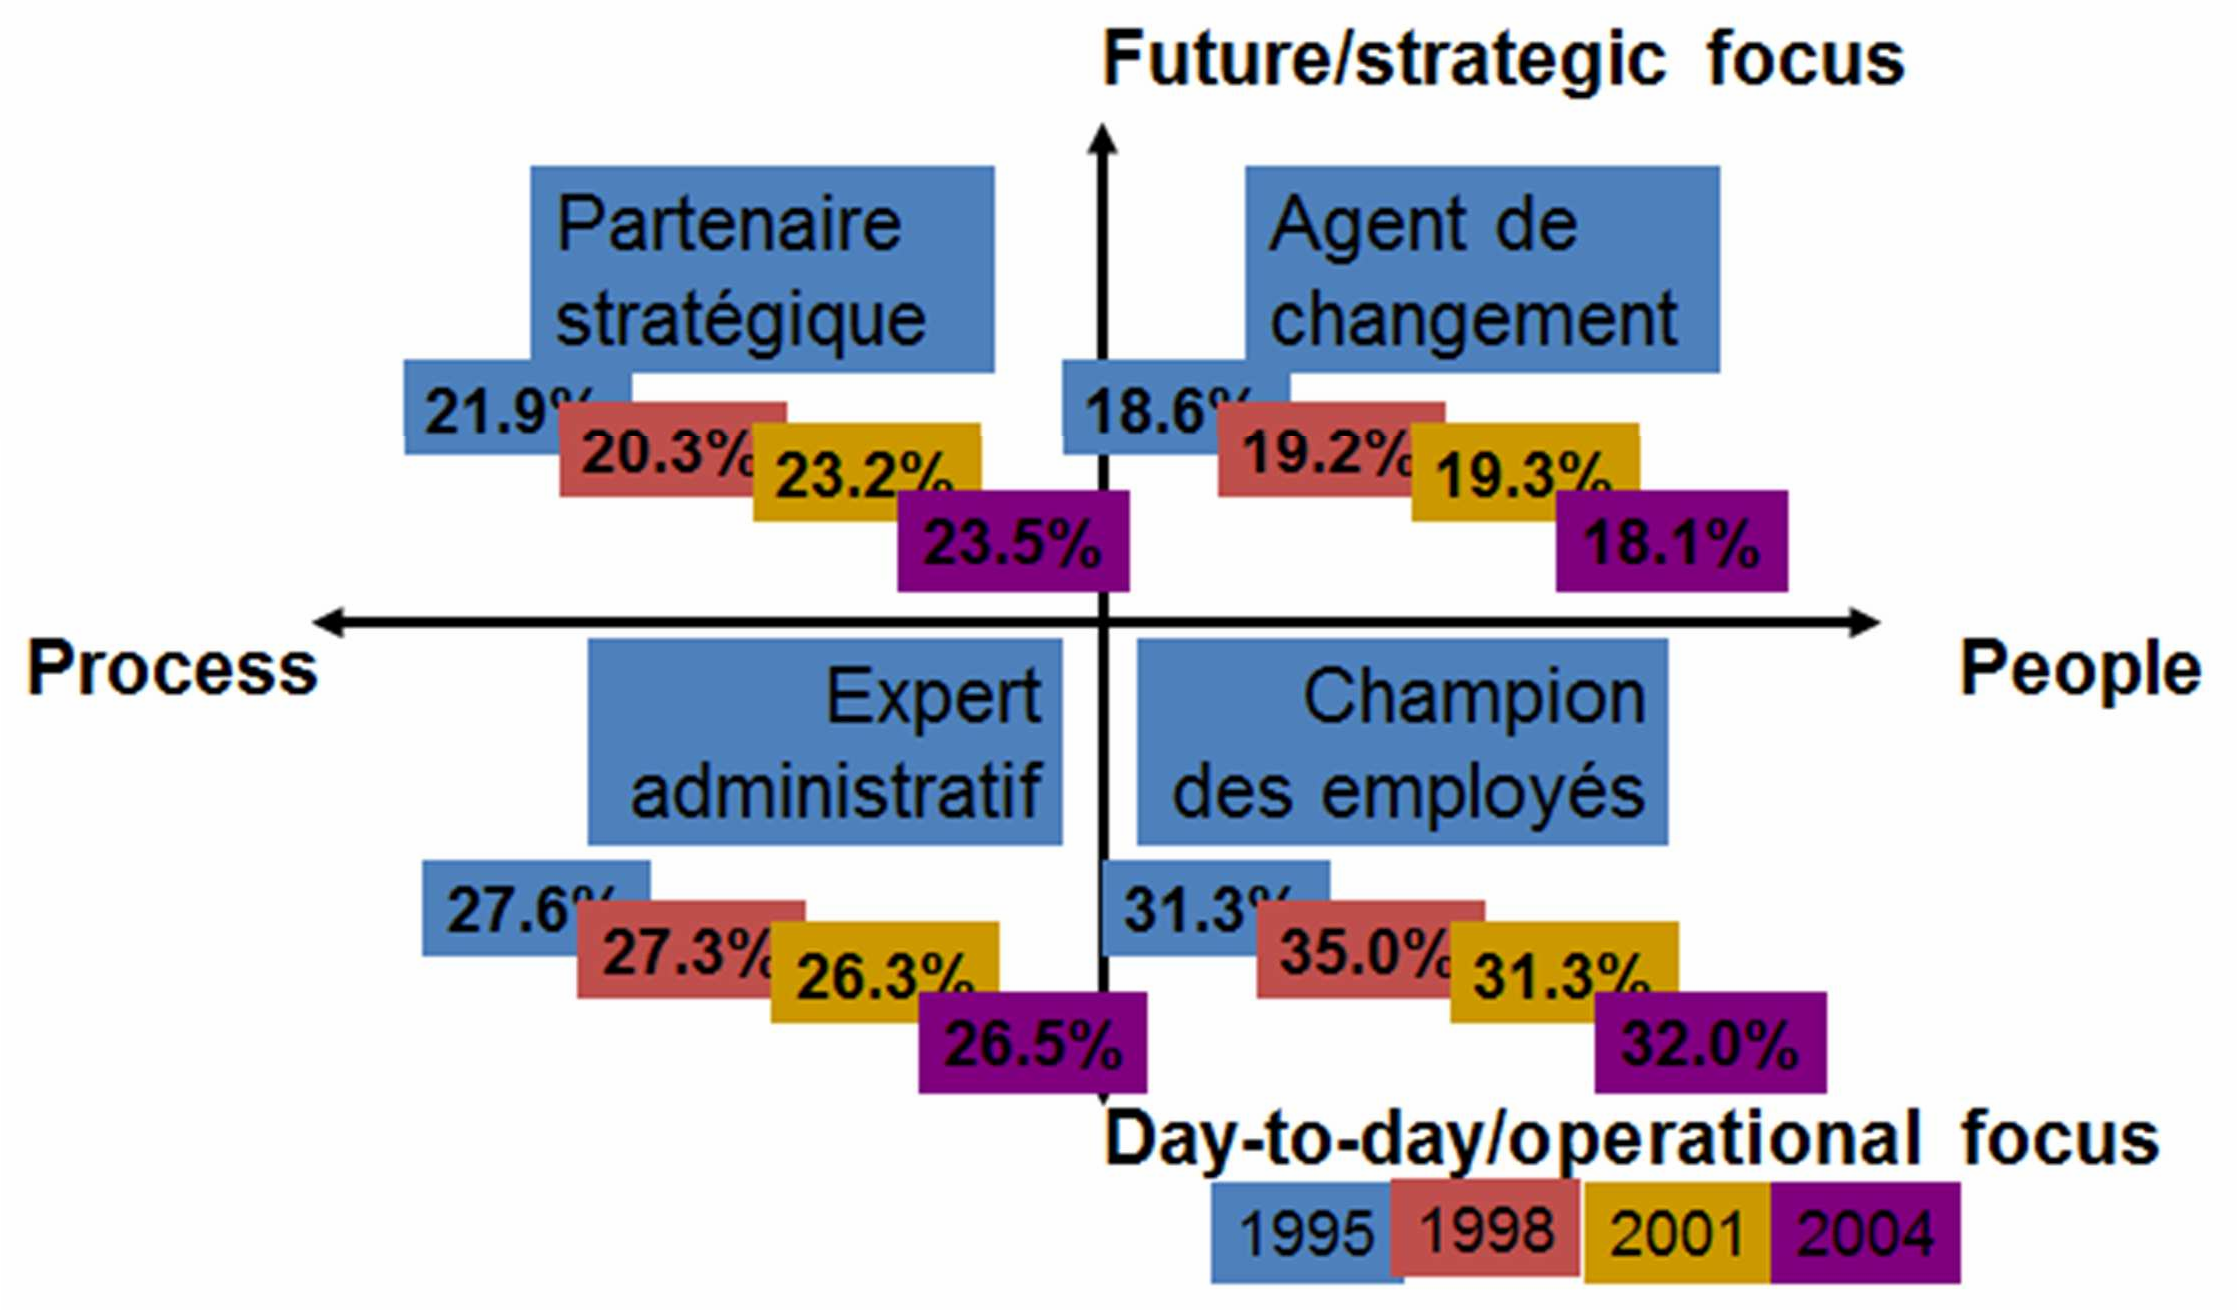
\includegraphics[width=\linewidth]{ulrich_pourcentage.png}

Le regard critique que nous pourrions développer face à son discours est que le rôle du DRH ne se limite pas uniquement à ce qu'il a raconté. En effet, son discours était très positif et basé sur l'innovation, le changement et l'humain. Cependant, son personnel étant hautement qualifié, on sait que celui-ci possède plus de pouvoir de négociation. Dès lors, son pouvoir diminue et il n'est probablement pas capable de faire tout ce dont il rêve. IBA est aussi une société côtée en bourse, ce qui implique qu'elle subit probablement des pressions de ses actionnaires, qu'elle a subit la crise financière mondiale de 2008 et cela n'a pas été abordé lors de la conférence alors que pour l'énorme majorité des entreprises, ça a causé des troubles internes important.

Le rôle du DRH pour l'avenir est d'être partie intégrante des organes de décision de l'entreprise pour assurer le bien-être et la pérennité des ressources humaines en leur assurant le bien-être psychologique, social et financier. Il faudra trouver des moyens de lier à nouveau l'homme à son entreprise pour éviter dans les sociétés à haut niveau de compétences de devoir former des personnes qui ne restent pas pour une longue période de temps. Il doit être à la fois administrateur et proche des attentes de ses employés.

\end{document}
